\documentclass[a4paper, 11pt, french]{report}
\usepackage[utf8]{inputenc}										% package désignant l'encodage
\usepackage[T1]{fontenc}	  									% je sais pas à quoi il sert
\usepackage[francais]{babel} 
\usepackage[colorlinks=true, urlcolor=blue, linkcolor=blue]{hyperref}
\usepackage{graphicx}
\usepackage{wrapfig}
\usepackage{multicol}


\author{Boncorps Robin \& Daniel Gwendal}
\title{Rapport de projet - FTP pair à pair}

\begin{document}
\maketitle

\chapter{Introduction} % lol
Dans le cadre de nos TP de réseaux, nous avons du développer une application client/serveur. Le but de ce projet est de comprendre les principes de fonctionnement des sockets, bases de toutes applications réseaux réparties. C'est dans cette optique que nous avons choisi de développer une application d'échange de fichiers en pair à pair. Nous allons donc, dans le présent rapport, présenter les différents protocoles et moyens utilisés pour mener à bien ce projet. Nous nous interesserons, par la suite, à la modélisation de l'application pour finir par présenter les différentes performances de l'application.

\chapter{Analyse}
Dans cette partie, nous allons présenter succintement les différentes bases sur lesquelles s'appuie l'application.

	\section{FTP : File Transfer Protocol} %robin
	FTP ou File Transfert Protocol est un protocol de communication destiné à l'échange de fichiers sur un réseau TCP/IP.
	FTP obéit à un modéle client-serveur, un client interrogant un serveur distant qui fonctionne sur la machine distante. (plus d'informations \url{http://fr.wikipedia.org/wiki/File_Transfer_Protocol})
		
	\section{Pair-à-pair} % gwendal
	Le pair-à-pair est un modèle de réseau informatique dans lequel tout client peut également être un serveur. On distingue deux types de réseaux pair-à-pair : les réseaux centralisés (les connexions se font par le biais d'un serveur) et décentralisés (les connexions se font directement entre clients). Ce type d'architecture est relativement connue du grand publique par le partage de fichiers, mais peut également servir au calcul scientifique ou à la communication. (plus d'informations \url{http://fr.wikipedia.org/wiki/Pair_%C3%A0_pair})
	
	\section{Application} % gwendal
	Une fois ces données en tête, nous avons trouvé que créer une application type FTP mais en réseau pair-à-pair était un défi intéressant. Afin de pouvoir tenir les délais du projet, nous avons décidé de mettre en place une architecture pair-à-pair centralisée, ce qui nous évitait de créer un protocole complexe de connaissance de voisins. Nous avons également estimé que pour une première version il était suffisant de ne permettre l'échange de fichier qu'entre deux stations (à l'inverse des protocoles utilisés par les trackers de torrents, qui récupèrent un même fichier de plusieurs endroits).
	\newline

	Notre application devait également permettre de gérer plusieurs connexions simultanées sur un même client (plusieurs demandes de fichiers, identiques ou non). Il était également évident qu'il fallait proposer les fonctionnalités de navigation propres à FTP (\emph{ls}, \emph{cd}, \emph{pwd}) afin de permettre la navigation et la récupération de fichiers.

\chapter{Modélisation}
	\section{Architecture} %gwendal
	Cette section détaillera plus précisement l'architecture retenue au niveau réseau. Comme nous l'avons dit précédement, nous avons choisi de développer une application pair-à-pair d'échange de fichier. Le schéma ci-dessous montre un cas d'utilisation basique de l'application.
	\begin{figure}[h!]
		\centering
		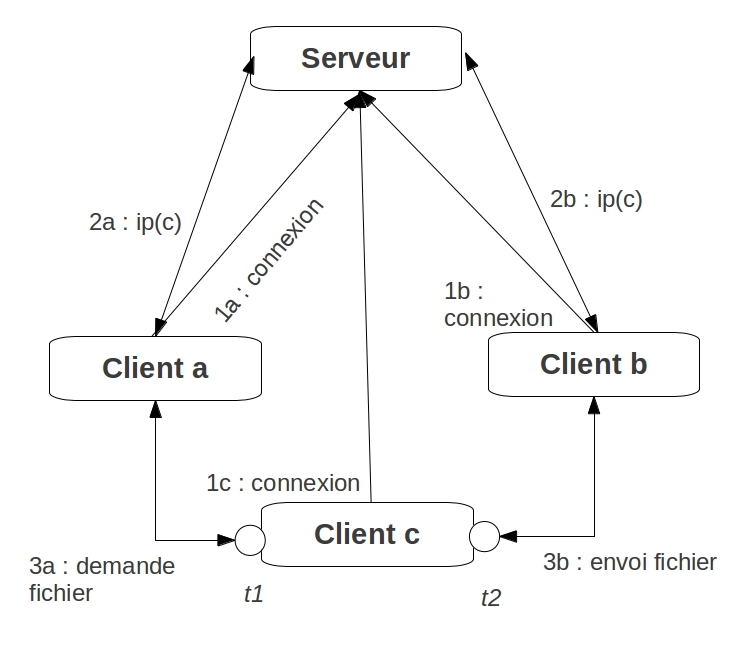
\includegraphics[scale=0.4]{archi.jpg}
		\label{Architecture générale}
	\end{figure}
	\newpage

	Dans cet exemple, on voit que les trois clients doivent dans un premier temps s'enregistrer auprès du serveur. Cette phase est nécessaire pour que le serveur puisse ensuite effectuer les résolutions d'adresses en fonctions des identifiants demandés. En effet, pour plus de sécurité et pour un meilleur confort d'utilisation, nous avons décidé que les clients ne devaient pas connaître les adresses ip de leurs contacts.
	\newline

	Dans notre exemple, les clients a et b demandent ensuite l'adresse ip du client c. Au niveau application, cette action est réalisée par une commande \emph{add\_friend<username>}. Le serveur résoud alors les adresses et renvoie l'adresse ip au client.
	\newline

	Enfin, les clients a et b se connectent au client c et commencent respectivement une récupération de fichier et un envoi (par les commandes \emph{get\_file<file name>} et \emph{put\_file<file name>}). On peut noter que le client c ouvre un thread par connexion, ce qui lui permet de traiter les deux demandes en parallèle.
	\newline
	Le serveur n'interragi plus dans les communications. Il ne sert qu'à résoudre des adresses.

	\textbf{Modélisation interne :} Nous n'avons pas voulu nous attarder sur la modélisation interne de l'application (diagramme de classes, explication détaillée \ldots) d'une part car le modèle retenu est très simple, et d'autre part car cet aspect ne nous semblait pas primordiale dans ce rapport. Voici néanmoins quelques points intéressants de la modélisation que nous avons retenu :
		~\\
		\begin{itemize}
			\item Une classe dédiée qui gère les envois et réceptions niveau socket (classe \emph{SocketManager})
			\item Une classe maintenant une réprésentation au niveau application d'une trame (aisée à manipuler) ainsi qu'un format particulier permettant un transfert facile (class \emph{Trame}).
			\item Enfin un ensemble de classes et de fonctions permettant de traiter la réception des messages (classe \emph{*handler})
		\end{itemize}
		~\\

		Cette modélisation orientée objet nous a permis d'accélérer le développement de l'application et de nous répartir intelligement les tâches.

	\section{PXP : Personal eXchange Protocol} %robin
		L'application permet d'échanger des fichiers grâce à son propre protocole (de la meme famille que ftp). 
		Ce protocole, que nous nommerons par la suite PXP pour Personal eXchange Protocol, permet le découpage/reconstruction d'un fichier entre 2 machines distante.
	
		\subsection{La trame PXP}
			\begin{figure}[!h]
				\centering
				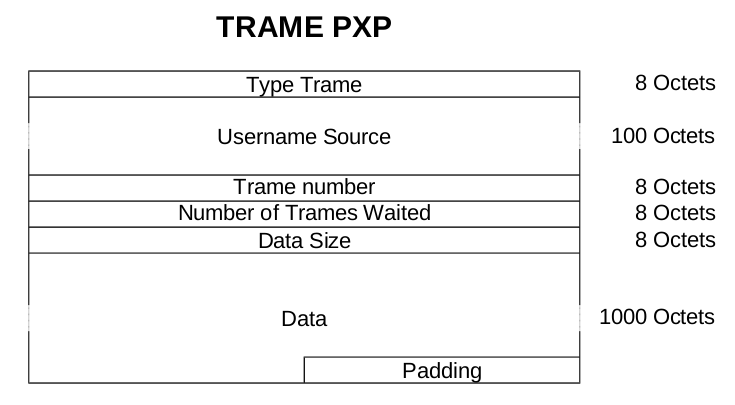
\includegraphics[scale=0.5]{TramePXP.png}
				\label{Trame PXP}
			\end{figure}
		
			Signification des champs :
			\begin{itemize}
				\item Type Trame : Le type de trame envoyé (nous détaillerons par la suite les différents types)
				\item Username Source : le nom de l'utilisateur qui envoi la trame
				\item Trame number : le numéro de la trame envoyée
				\item Number of Trame Waited : le nombre de trames attendues pour avoir tout le fichier
				\item Data Size : la taille effective des données comprises dans la partie Data
				\item Data : les données (une partie du fichier)
				\item Padding : 0 ajoutés pour remplir le champ Data
			\end{itemize}
			
			\subsubsection{Type Trame}
				Chaque action effectuée sur une machine distante a un type particulier
				\begin{itemize}
					\item CON\_SERV : demande de connexion au server
					\item ACK\_CON : le serveur accepte votre connexion
					\item DEM\_AMI : demande d'ami pour echange pair à pair
					\item DEM\_CON\_AMI : demande d'établissement d'une connexion avec autre client distant
					\item CHECK\_CON : vérification que le client distant est connecté
					\item CMD\_CON : initialisation du mode commande 
					\item CMD\_HOME : le path home du client distant est envoyé
					\item CMD : envoi d'une commande
					\item LS\_RET : retour d'une commande LS
					\item CD\_RET : retour d'une commande CD
					\item MAJ\_PATH : mise à jour du path courant
					\item CMD\_END : fin du mode commande
					\item DEM\_FIC : demande d'envoi d'un fichier
					\item ENV\_FIC : envoi du fichier
					\item ACK : acquittement de reception du fichier
					\item FIN\_CON\_AMI : fin de connection avec le client distant
					\item FIN\_CON\_SERV : fin de connexion avec le serveur
					\item ERROR : Trame d'erreur sur le client distant
				\end{itemize}
			
			
		\subsection{Transfert de données}
			Lors de l'envoi d'un fichier, si sa taille dépasse la taille maximum des datas d'une trame (1000 Octets ici), le fichier doit être découpé en plusieurs partie. 
			Ceci se fait tout simplement en parcourant le fichier par bloc de 1000 octets et en envoyant directement une trame contenant ces données.
			Il faut toute fois noter qu'il faut tout d'abord connaître la taille du fichier pour déterminer le nombre de trames qui vont être envoyées.
			On determine donc le nombre de trame a envoyer ainsi que la taille des données qui seront contenues dans la dernière trame (qui peut ne pas être complete)
			
			
			La reconstruction du fichier par ecriture direct des données contenues dans les trames reçues dans le fichier destination. Lors de la reception de la première trame du fichier, le nombre de trame attendu est extrait et permet de savoir combien de trame sont encore à recevoir. 
			Toutefois, la reception des trames du fichier s'arretera si l'ordre n'est pas respecté. Ceci n'est pas sensé arriver car TCP gère déjà l'ordre d'arrivé des trames avec son propre système.
			
\chapter{Résultats}
	\section{Vitesses de transfert}  %gwendal
	Nous n'avons pas eu le temps de récupérer un ensemble de données précises sur l'utilisation de l'application. Néanmoins nous pouvons donner des ordres de grandeurs sur les vitesses de transfert : 
		~\\
		\begin{itemize}
			\item Fichier de petite taille (< 1mo) : entre 0 et 2 secondes.
			\item Fichier de taille moyenne ( 100mo - 500 mo) : entre 10 et 20 secondes.
			\item Fichier de taille imposante (1go) : entre 30 secondes et 1 minute.
		\end{itemize}
		~\\

	Les tests ont été réalisés pour le premier cas sur différents fichier pdf que nous avions à disposition (rapports de projets précédents, articles \ldots), le test du fichier de taille moyenne a été réalisé pendant la démonstration de travaux pratique avec une fichier pdf d'environ 140 mo, enfin le test de fichier imposant à été réalisé avec une image iso ubuntu.
	\newline

	Nous sommes relativement content de la vitesse obtenue. Il ne faut néanmoins pas oublier que ces résultats sont dépendant de la charge et de la performance du réseau, qui n'ont pas beaucoup influé sur les tests (réseau de deux machines ou réseau local en salle de travaux pratiques).
	\newline

	Une des expications de cette vitesse est l'absence de contrôle d'erreur type CRC, nous n'en avons en effet pas eu besoin puisque le protocole TCP utilisé au travers des sockets assure l'intégrité des données.

	De la même façon nous n'avons pas eu à réordonner les trames arrivant, puisque nous avons opté pour des sockets en mode connecté, qui nous garantissait l'ordre d'arrivée des trames.

	\section{Format de trames} %robin
	Nous avons opté pour une taille de trame de 1132 octets (entête comprise) pour ne pas dépasser la taille maximale des données d'une segment de TCP qui est 1500 octets. Ceci permet de ne pas avoir a redécouper les données envoyées, ce qui ralentirait la vitesse de transfert.
	

\chapter{Conclusion}
	\section{Apports} %gwendal
	Ce projet de travaux pratiques nous a permis de nous familiariser avec la programmation d'une application réseau, qui plus est distribuée. Nous avons pu apprendre à manipuler les sockets et conforter notre utilisation des threads.
	\newline

	D'un point de vue personnel, nous avons aimé travailler sur un système pair-à-pair, qui est une approche bien particulière du développement d'application. Nous regrettons simplement de ne pas avoir eu plus de temps à y consacrer afin d'effectuer de meilleurs tests ou encore d'offrir une interface ergonomique et intuitive pour l'utilisateur.


	\section{Difficultés rencontrées} %robin
	Nous avons principalement rencontré des difficultés lors du découpage des fichiers ainsi qu'au niveau de la procedure de reception de trame. 
	La première difficulté était de savoir comment découper un fichier et de le reconstruire après.
	La deuxième difficulté était que, lors de la reception de toutes les trames contenant le fichier, le système s'arrêtait. Ce problème était du à l'utilisation de la fonction read dans un socket pour récupérer son contenu. En effet, cette fonction n'attend pas que le buffer de reception soit rempli, ce qui entrainait une perte d'information. La solution apporté a été d'utiliser la fonction recv qui permet, grâce à un flag, d'attendre que le buffer soit rempli avant de recevoir une autre trame. 
\end{document}
